\documentclass{beamer}

\usepackage[size=custom,width=86.36,height=111.76,orientation=portrait,scale=1.8]{beamerposter}
\usetheme{LLT-poster}
\usecolortheme{Entrepreneur}

\usepackage[utf8]{inputenc}
\usepackage[T1]{fontenc}
\usepackage{libertine}
\usepackage[scaled=0.92]{inconsolata}
\usepackage[libertine]{newtxmath}
\usepackage{wrapfig}
\usepackage{mathtools}
\usepackage{calc}
\usepackage{mwe}

\usepackage{hyperref}
\hypersetup{
    colorlinks=true,       % false: boxed links; true: colored links
    urlcolor=cyan           % color of external links
}

\usepackage{tikz}

\usepackage{xcolor}

\definecolor{mediumelectricblue}{rgb}{0.01, 0.31, 0.59}
\definecolor{midnightblue}{rgb}{0.1, 0.1, 0.44}
\definecolor{azure(colorwheel)}{rgb}{0.0, 0.5, 1.0}
\definecolor{babyblueeyes}{rgb}{0.63, 0.79, 0.95}
\definecolor{mayablue}{rgb}{0.45, 0.76, 0.98}
\definecolor{spirodiscoball}{rgb}{0.06, 0.75, 0.99}
\definecolor{brandeisblue}{rgb}{0.0, 0.44, 1.0}
\definecolor{dodgerblue}{rgb}{0.12, 0.56, 1.0}

\usepackage{listings}

\newcommand\JSONnumbervaluestyle{\color{blue}}
\newcommand\JSONstringvaluestyle{\color{blue}}

\newif\ifcolonfoundonthisline

\makeatletter

\lstdefinestyle{json}
{
  showstringspaces    = false,
  alsoletter          = 0123456789.,
  morestring          = [s]{"}{"},
  stringstyle         = \ifcolonfoundonthisline\JSONstringvaluestyle\fi,
  MoreSelectCharTable =%
    \lst@DefSaveDef{`:}\colon@json{\processColon@json},
  basicstyle          = \ttfamily\small,
  keywordstyle        = \ttfamily\bfseries,
}

\newcommand\processColon@json{%
  \colon@json%
  \ifnum\lst@mode=\lst@Pmode%
    \global\colonfoundonthislinetrue%
  \fi
}

\lst@AddToHook{Output}{%
  \ifcolonfoundonthisline%
    \ifnum\lst@mode=\lst@Pmode%
      \def\lst@thestyle{\JSONnumbervaluestyle}%
    \fi
  \fi
  \lsthk@DetectKeywords% 
}

\lst@AddToHook{EOL}%
  {\global\colonfoundonthislinefalse}

\usebackgroundtemplate{\tikz\node[opacity=0.1]{\includegraphics[width=\paperwidth,height=\paperheight]{img/world.png}};}

\title{\raisebox{\heightof{B)}-\height+7mm}{
\includegraphics[height=1.3em]{img/beacon-network-short.png}}Beacon Network: A System for Global Genomic Data Sharing}
\author{M. Cupak, M. Fiume, V. Rockai, S. Keenan, D. Lloyd, P. Goodhand}
\footimage{\includegraphics[width=2.1em]{img/ga4gh.png}}

\begin{document}
\begin{frame}[fragile]

\begin{columns}[T]
\begin{column}{.46\textwidth}

\begin{block}{Motivation\hfill\raisebox{\heightof{B)}-\height+2pt}{\includegraphics[height=1em]{img/idea.png}}}
\begin{itemize}
\item Analysis of large volumes of genomic data has the potential to drive discoveries and applications in medicine.
\item No institution has enough resources to capture all human variation.
\item A global federated network of shared genomic data is needed.
\end{itemize}
\end{block}

\begin{block}{Beacon\hfill\raisebox{\heightof{B)}-\height+2pt}{\includegraphics[height=1em]{img/logo.png}}}
\begin{itemize}
\item Standard defining a \color{brandeisblue} web service \color{black} for \color{brandeisblue} discovery \color{black} and \color{brandeisblue} sharing \color{black} of information about alleles.
\item API:
	\begin{itemize}
	\item Request: \textit{Do you have information about this mutation?}
	\item Response: \textit{Yes/No (and optionally additional information).}
	\end{itemize}
\item Initiative of the Global Alliance for Genomics \& Health.
\item More information: \url{https://ga4gh.org/#/beacon}.
\end{itemize}
\end{block}

\begin{block}{Beacon Network\hfill\raisebox{\heightof{B)}-\height+2pt}{
\includegraphics[height=1em]{img/beacon-network-short.png}}}
\begin{itemize}
\item \color{brandeisblue}Search engine \color{black} across the world's beacons.
\item Translates genomic queries for each beacon, intelligently distributes the queries through the network, and aggregates the results.
\item API:
	\begin{itemize}
	\item Request: \textit{Who has information about this mutation?}
	\item Response: \textit{List of beacons and their responses.}
	\end{itemize}

\vspace{5mm}
\begin{center}
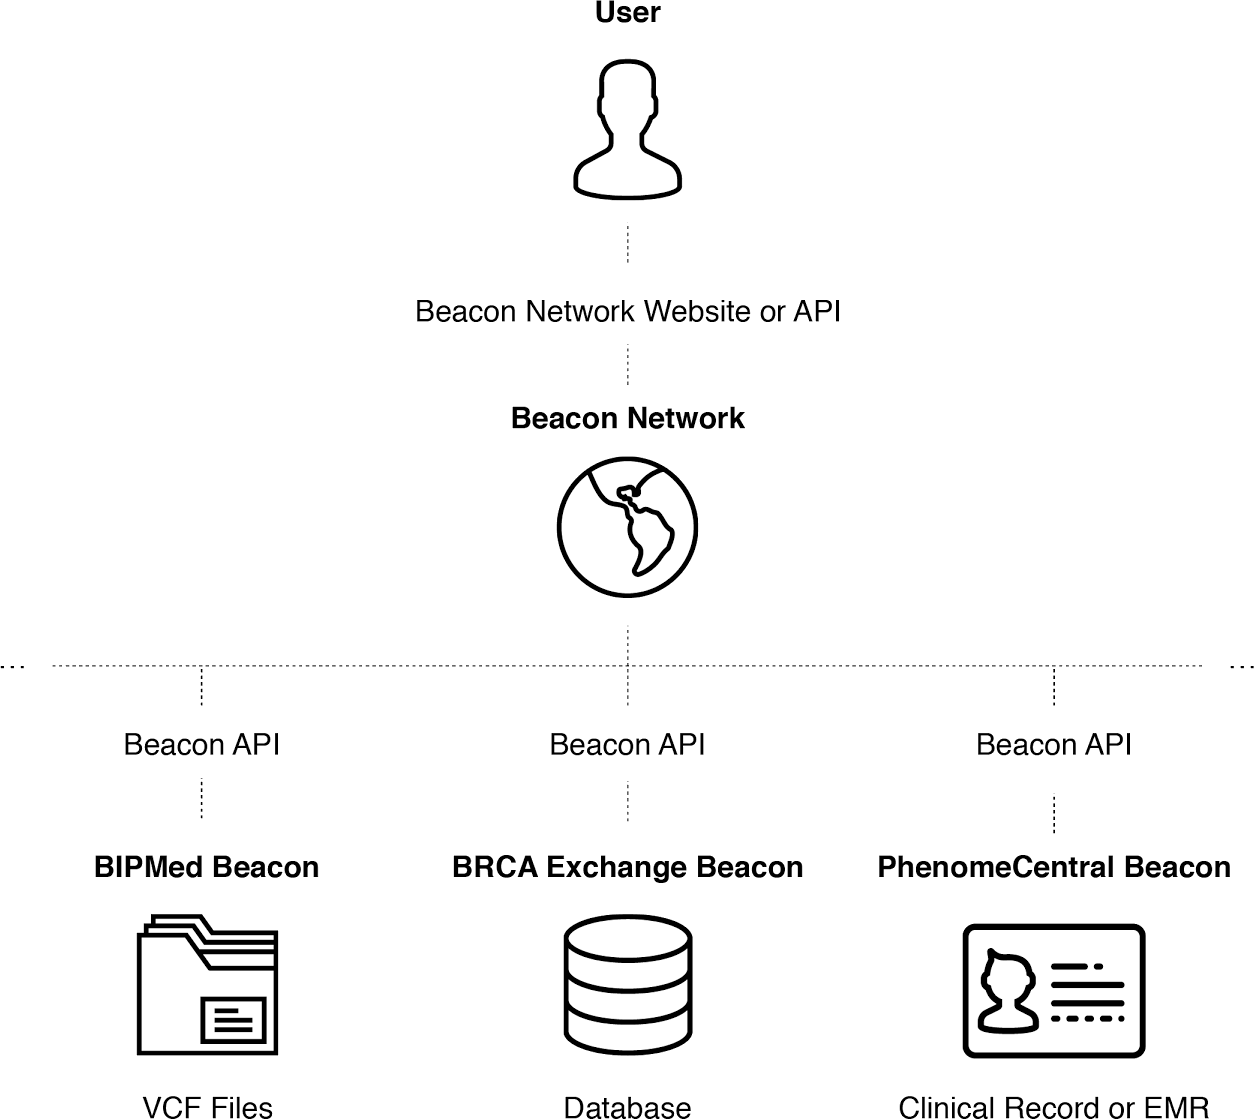
\includegraphics[width=\linewidth]{img/schema-without-text.png}
\end{center}
\vspace{2mm}

\item Provides REST API, web client, command line client, query library, compatible beacon implementations in multiple programming languages, and adapters for various sources of genomic data.
\item More information: \url{http://beacon-network.org}.
\end{itemize}
\end{block}
\end{column}


\begin{column}{.46\textwidth}
\begin{block}{User interface\hfill\raisebox{\heightof{B)}-\height+2pt}{\includegraphics[height=1em]{img/usage.png}}}
\begin{center}
\includegraphics[width=\linewidth]{img/client-long.png}
\vspace{-2mm}
\end{center}
\end{block}

\begin{block}{Adoption\hfill\raisebox{\heightof{B)}-\height+2pt}{\includegraphics[height=1em]{img/adoption.png}}}
\begin{itemize}
\item 25+ of the world's top genomic organizations, 60+ beacons.

\vspace{2mm}
\begin{center}
\includegraphics[width=\linewidth]{img/map.png}
\end{center}
\item Served 400K+ queries from 6K+ users in 100+ countries, resulting in 2M+ queries dispatched to the participants of the network.

\vspace{2mm}
\begin{center}
\includegraphics[width=\linewidth]{img/queries.png}
\end{center}
\end{itemize}
\end{block}
\end{column}

\end{columns}
\end{frame}
\end{document}